\begin{figure}[htbp]
	\centering
	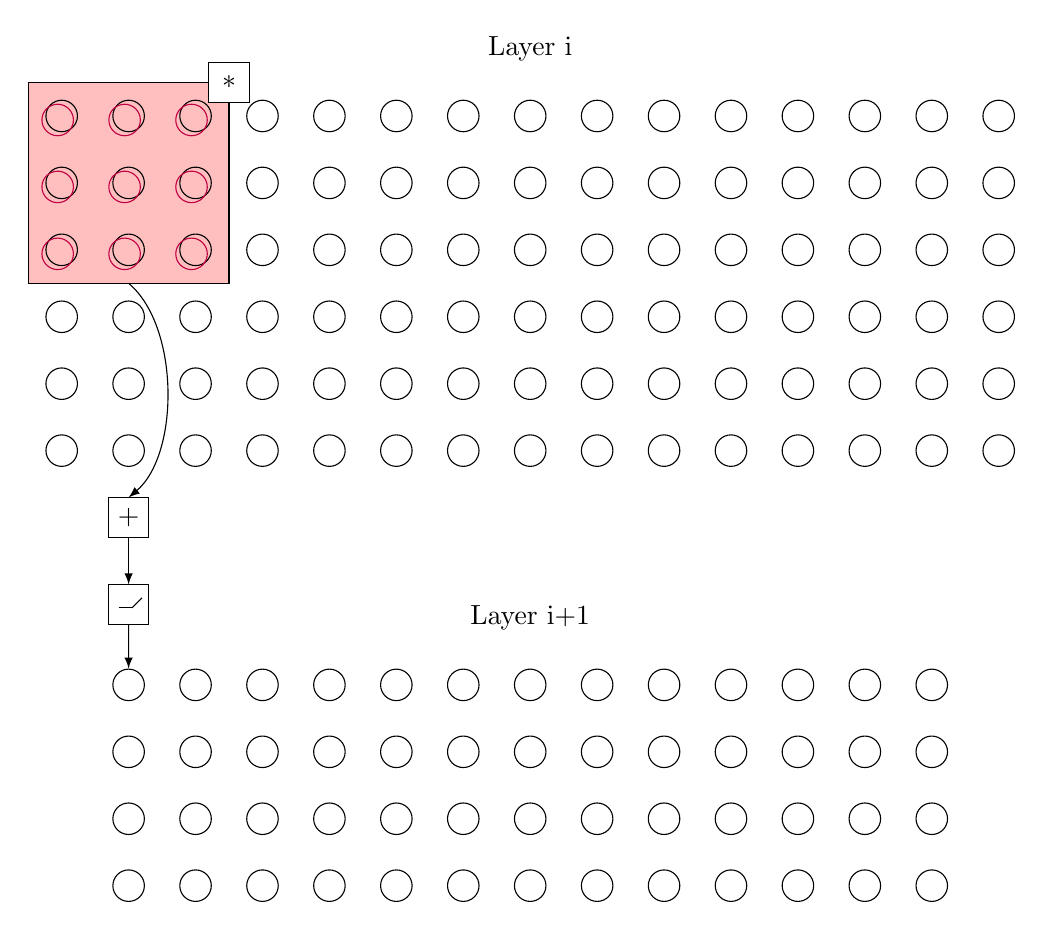
\begin{tikzpicture}[scale=0.85,every path/.style={>=latex}]
		\node (layeri) at (7,6) {Layer i};
		\node (layeri) at (7,-2.5) {Layer i+1};
     	
     	% draw background for filter
     	\draw[fill=pink] (-0.5,5.5) rectangle (2.5,2.5);
     	
     	% draw rectangle with "*" inside
     	\draw[fill=white] (2.2,5.8) rectangle (2.8,5.2);
     	\node at (2.5,5.5) {$*$};
     	
     	
     	% draw layer 1
     	\foreach \x in {0,...,14}
     	{
     		\foreach \y in {0,...,5}
     		{
     			\node(1-\x-\y) at (\x,\y) [circle,draw,minimum size=0.4cm] {};
     		}
     	}
     	
     	% draw layer 2
     	\foreach \x in {1,...,13}
     	{
     		\foreach \y in {1,...,4}
     		{
     			\node(2-\x-\y) at (\x,\y - 7.5) [circle,draw,minimum size=0.4cm] {};
     		}
     	}
     	
     	%draw filter
     	\foreach \x in {0,...,2}
     	{
     		\foreach \y in {3,...,5}
     		{
     			\node(f-\x-\y) at (\x - 0.06,\y - 0.06) [circle,draw,purple,minimum size=0.4cm] {};
     		}
     	}
     	
     	% draw line from filter to "+" rectangle
     	\draw[->,looseness=0.8,out=320,in=40] (1.,2.5) to (1.,-0.7);
     	
     	% draw "+" rectangle
     	\draw[fill=white] (0.7,-0.7) rectangle (1.3,-1.3);
     	\node at (1,-1) {$+$};
     	
     	% draw line from "+" rectangle to ReLU rectangle
     	\draw[->] (1,-1.3) to (1,-2.);
     	
     	% draw ReLU rectangle
     	\draw[fill=white] (0.7,-2.) rectangle (1.3,-2.6);
     	\draw[->] (1,-2.6) to (2-1-4);
     	\draw[-] (0.85,-2.35) to (1.05,-2.35);
     	\draw[-] (1.05,-2.35) to (1.2,-2.2);
	\end{tikzpicture}
	\caption{Functioning of a convolutional layer}
	\label{fig:centered_filter}
\end{figure}
